\section{Логистичка регресија}

Со овој алгоритам ќе изградиме модел за логистичка регресија кој ќе предвидува
дали кандидатот е примен или не на универзитет.

Вие сте раководител на некој оддел во универзитет и сакате да ги одредите
шансите на кандидатот да биде примен во зависност од неговите резултати на двата
приемни испити. Поседувате податоци од претходните уписи со резултатите од двата
испити и одлуката дали е примен кандидатот или не.

Целта е да се изгради модел за класификација кој ќе ја предвидува веројатноста
за да биде примен кандидатот во зависност од резултатите од двата испити.

\subsection{Визуелизација на податоците}
На слика \ref{fig:plot2} е прикажана визуелизација на податоците од податочното
множество, во кое со жолти кругчиња се означени одбиените, а со црвени плус
знаци примените кандидати.

\begin{figure}[htb]
\centering
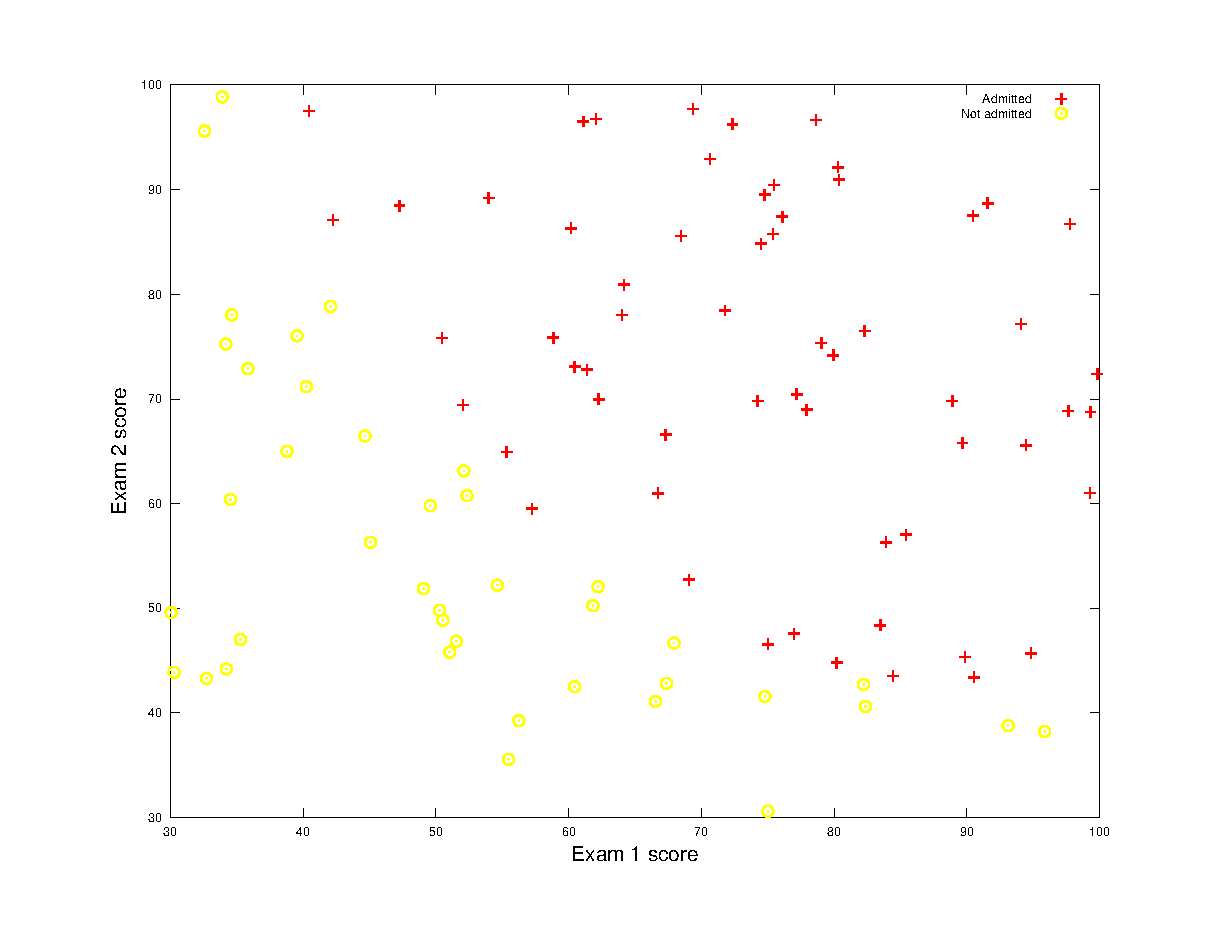
\includegraphics[width=.9\textwidth]{src/logisticRegression/data}
\caption{Scatter plot на податочното множество}
\label{fig:plot2}
\end{figure}

\lstinputlisting[firstline=9,lastline=16,caption=Разделување на податочното
множество на позитивни и негативни примероци и негова визуелизација]{src/logisticRegression/plotData.m}

\subsection{Имплементација}

\subsubsection{Sigmoid функција}

Хипотезата во логистичка регресија е дефинирана со:

\[
	h_{\theta}(x) = g(\theta^Tx),
\]
каде функцијата $g$ e sigmoid функцијата. Sigmoid функцијата е дефинирана со:

\[
	g(z) = \frac{1}{1 + e^{-z}}
\]

\lstinputlisting[firstline=5,lastline=6,caption=Имплементација
на функцијата sigmoid]{src/logisticRegression/sigmoid.m}

Функцијата на чинење во логистичка регресија е:

\subsubsection{Функција на чинење и градиент}
\[
	J(\theta) = \frac{1}{m}\sum^m_{i=1} \left[ -y^{(i)} \log(h_\theta(x^{(i)})) -
	(1 - y^{(i)})\log(1 - h_\theta(x^{(i)})) \right]
\]

а градиентот на чинење е вектор со иста должина како $\theta$ каде што $j^{th}$
елемент (за $j = 0, 1, \ldots ,n$) е дефиниран на следниот начин:
\[
	\frac{\partial J(\theta)}{\partial\theta_j} =
	\frac{1}{m}\sum^m_{i=1}{(h_\theta(x^{(i)}) - y^{(i)})}x^{(i)}_j
\]

\subsubsection{Учење на параметрите со \texttt{fminunc}}
Учењето на параметрите $\theta$ во овој алгоритам ќе го правиме со употреба со
готовата функција за минимизација \texttt{fminunc}. Ова е вградена функција која
наоѓа минимум на неограничена \footnote{Ограничувањата во оптимизацијата често се однесуваат на ограничувања на
параметрите, на пример, ограничувања на вредностите на $\theta$ (пр., $\theta
<= 1$). Логистичката регресија нема такви ограничувања затоа што $\theta$ може
да ја прими вредноста на секој реален број.} функција.

За логистичка регресија ја оптимизираме функцијата на чинење $J(\theta)$ со
параметар $\theta$.

Конкретно, ќе ја користиме fminunc да ги пронајдеме најдобрите параметри
$\theta$ за функцијата на чинење на логистичката регресија, за дадено податочно
множество (X и y вредности). Функцијата fminunc ќе ја повикаме со следните
аргументи:
\begin{itemize}
  \item Иницијалните вредности на параметрите кои сакаме да ги оптимизираме.
  \item Функција, која за дадено тренинг податочно множество и дадено $\theta$,
  пресметува функција на чинење на логистичка регресија и градиент.
\end{itemize}

\lstinputlisting[firstline=50,lastline=58,caption=Повикување
на функцијата за оптимизација
\texttt{fminunc}]{src/logisticRegression/logisticRegression.m}

Со овој код фрагмент, најпрво ги дефинираме опциите со кои ќе ја повикаме
\texttt{fminunc}. Со поставување на \texttt{GradObj} на \texttt{on}, ѝ
кажувме на \texttt{fminunc} дека нашата функција враќа и чинење и градиент.
Ова овозможува \texttt{fminunc} да го користи градиентот за минимизирање на
функцијата. Со поставување на \texttt{MaxIter} на 400, ја ограничуваме
\texttt{fminunc} да се извршува максимум 400 итерации.

\begin{figure}[htb]
\centering
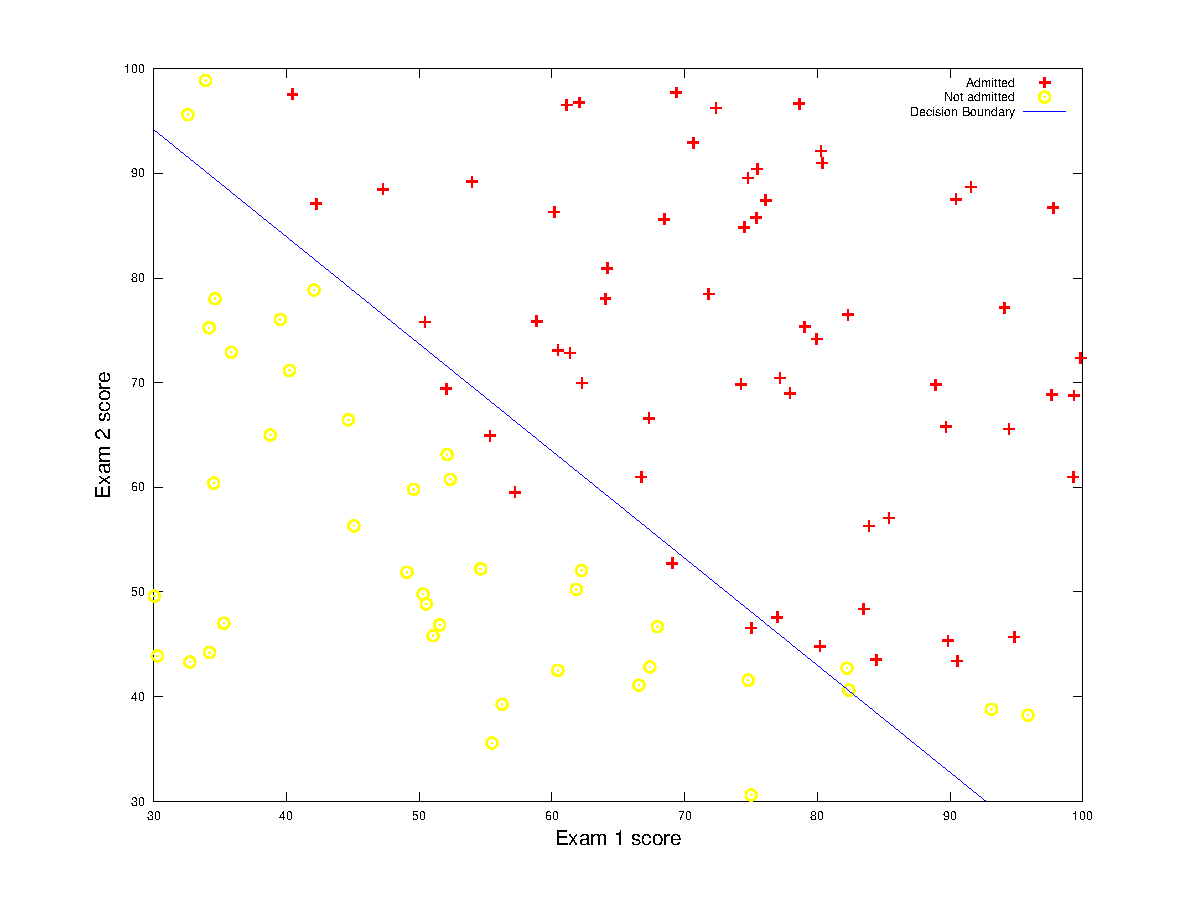
\includegraphics[width=.9\textwidth]{src/logisticRegression/decisionBoundary}
\caption{Податочното множество со границата на одлука}
\label{fig:decisionBoundary}
\end{figure}

Вредноста на $\theta$ која се добива како резултат на оптимизацијата служи за
исцртување на границата на одлука прикажана на слика \ref{fig:decisionBoundary}.

\subsubsection{Евалуација на логистичката регресија}

Откако ќе ги научиме параметрите, го користиме моделот за да предвидиме дали
одреден кандидат ќе биде примен. За кандидат кој на првиот испит имал 45 поени,
а на вториот 85, добиваме веројатност за успех од 0.776.

Нашиот модел го евалуираме на целото тренинг множество.

\lstinputlisting[firstline=7,lastline=10,caption=Функцијата
за евалуација на тренинг множеството]{src/logisticRegression/predict.m}